\documentclass[runningheads,a4paper]{llncs}
% proper encoding
\usepackage[T1]{fontenc}

% autoref command
\usepackage[pdftex,urlcolor=black,colorlinks=true,linkcolor=black,citecolor=black]{hyperref}

% better typography
\usepackage[activate=compatibility]{microtype}

% graphics
\usepackage{graphicx}

\usepackage[lofdepth,lotdepth]{subfig}

% URLs
\usepackage{url}

\begin{document}

\mainmatter

\title{Enriching Content Objects for Multimodal Search with Data from the Linking Open Data Cloud}
\authorrunning{Enriching Content Objects for Multimodal Search with LOD Cloud Data}

\author{Jonas Etzold\inst{1} \and Thomas Steiner\inst{2} \and Arnaud Brousseau\inst{2}\thanks{The author was an intern at Google Germany GmbH at time of core development.} \and Paul Grimm\inst{1}}

\institute{\label{fulda}Hochschule Fulda, Marquardstr. 35
36039 Fulda, Germany\\
\urldef{\emails}\path|{jonas.etzold,paul.grimm}@hs-fulda.de|\emails\\
\and Google Germany GmbH, ABC-Str. 19, 20355 Hamburg, Germany\\
\urldef{\emails}\path|{tomac,arnaudb}@google.com|\emails\\
}

\maketitle

\setcounter{footnote}{0}

\begin{abstract}
In this paper, we report on the \mbox{I-SEARCH} EU (FP7 ICT STREP) project
whose objective is the development of a~multimodal search engine that supports multimodal
in- and output, as well as multimodal query refinement.
An important aspect for \mbox{I-SEARCH} to work is the so-called
\emph{Rich Unified Content Description} \emph{\mbox{(RUCoD)}} format
consisting of a~multi-layered structure
for the description of low and high level features of content objects.
The \emph{\mbox{(RUCoD)}} description format allows content objects
to be queried in a~consistent way by using extracted \mbox{\emph{RUCoD}} features.
For the fully automatic or the supervised creation of content objects,
we have developed a tool called \mbox{\emph{CoFetch}}
that retrieves part of its data from the Linking Open Data cloud.
During the session, we will present a~live demonstration of the \mbox{I-SEARCH}
Graphical User Interface (GUI) and the \mbox{\emph{CoFetch}} tool, and,
via pre-defined use cases, show how we imagine multimodal search in the future.
We are looking for networking opportunities with projects dealing with
semantic annotation of large-scale multimedia archives and 
projects interested in our \emph{RUCoD} feature extraction techniques.
\end{abstract}

\section{Introduction}
Search engines over the years have coined a~common interaction pattern:
the search box.
We enhance this interaction pattern by context-aware modality input toggles
that create modality query tokens in the \mbox{I-SEARCH} search
box\footnote{See \url{http://isearch.ai.fh-erfurt.de/} for a~live demonstration.}.
The concept-centered \mbox{I-SEARCH} search engine lets users search
by using different modalities and combinations of modalities.
Supported modalities and combinations thereof are \emph{audio}, \emph{video},
\emph{rhythm}, \emph{image}, \emph{3D object}, \emph{sketch}, \emph{emotion},
\emph{social signals}, \emph{geolocation}, and \emph{text}.
For example, in order to get a~holistic view on the concept of
Leonardo da Vinci's painting of the \emph{Mona Lisa} (also known as \emph{La Joconde}),
a~user could search by uploading a~photograph of the painting,
and---besides the obvious textual description---also get back
the geolocation of the Louvre museum,
a~video of a~relevant section of a~Louvre museum walk,
or the audio recording of an explanation of the painting.

\begin{figure}
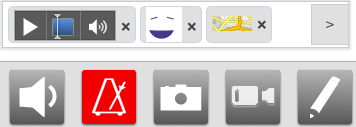
\includegraphics[width=.1\linewidth]{ui.png}
\caption{\mbox{I-SEARCH} with 3 modality query tokens \emph{audio}, \emph{emotion}, and \emph{geolocation}.}
\label{fig:ui}
\end{figure}


\section{Rich Unified Content Description (RUCoD)}
In order to allow for the before-mentioned concept-centeredness,
in the context of \mbox{I-SEARCH}, we have first introduced
the concept of so-called \emph{content objects}, and second,
a~description format named \emph{Rich Unified Content Description
\mbox{(RUCoD)}}~\cite{ijmis2010}.
Content objects are rich media presentations, enclosing different types of media,
along with real-world information and user-related information.
\mbox{\emph{RUCoD}} provides a~uniform descriptor for all types of content objects,
irrespective of the underlying media and accompanying information.
In the following Section, we will introduce a tool called \mbox{\emph{CoFetch}},
which serves for the fully automatic or the supervised creation of content objects.

\begin{figure}[]
  \centering
    \subfloat[][Architecture of the CoFetch tool.]{
      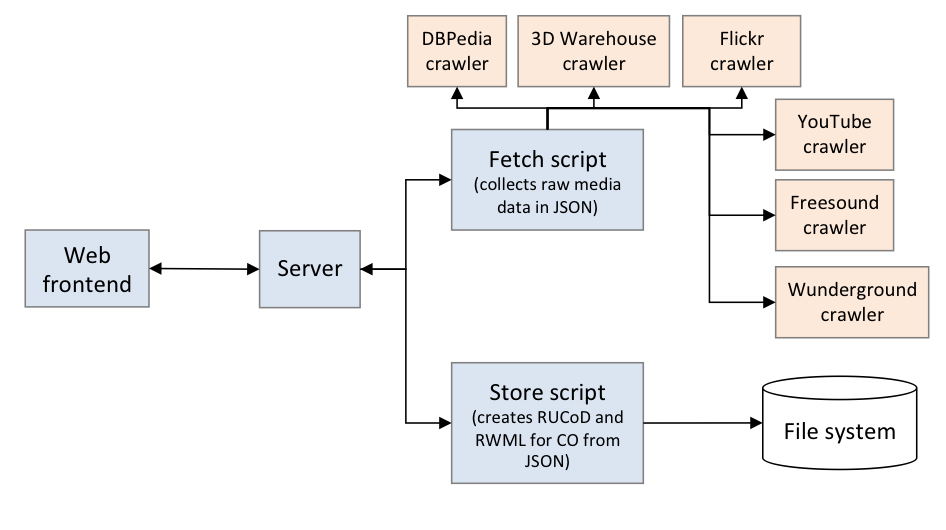
\includegraphics[width=0.5\textwidth]{architecture.png}
      \label{fig:architecture}}
    \qquad
    \subfloat[][Screenshot of the CoFetch tool.]{
      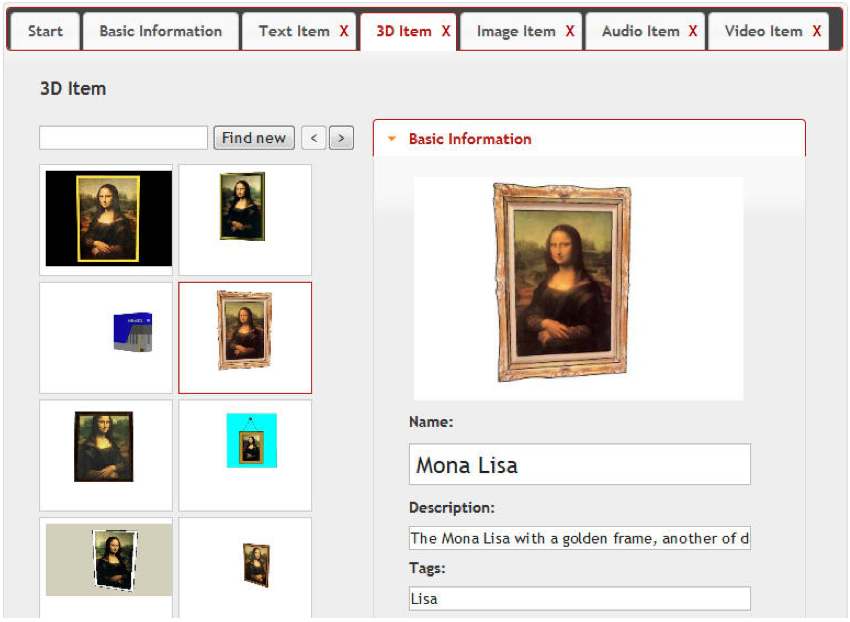
\includegraphics[width=0.4\textwidth]{screenshot.png}
      \label{fig:screenshot}}
\caption{CoFetch.}
\label{fig:cofetch}
\end{figure}

\bibliographystyle{splncs03}
\bibliography{eswc2012}

\end{document}